%%\documentclass[a4paper,12pt,oneside]{llncs}
\documentclass{book}
%\usepackage[right=2cm,left=3cm,top=2cm,bottom=2cm,headsep=0cm]{geometry}

%%%%%%%%%%%%%%%%%%%%%%%%%%%%%%%%%%%%%%%%%%%%%%%%%%%%%%%%%%%
%% Juego de caracteres usado en el archivo fuente: UTF-8
\usepackage{ucs}
\usepackage[utf8x]{inputenc}
%\usepackage{eurosym}

%%%%%%%%%%%%%%%%%%%%%%%%%%%%%%%%%%%%%%%%%%%%%%%%%%%%%%%%%%%
%% Juego de caracteres usado en la salida dvi
% Otra posibilidad: \usepackage{t1enc}
\usepackage[T1]{fontenc}

%%%%%%%%%%%%%%%%%%%%%%%%%%%%%%%%%%%%%%%%%%%%%%%%%%%%%%%%%%%
%% Ajusta maergenes para a4
\usepackage{a4wide}

%%%%%%%%%%%%%%%%%%%%%%%%%%%%%%%%%%%%%%%%%%%%%%%%%%%%%%%%%%%
%% Uso fuente postscript times, para que los ps y pdf queden y pequeños...
\usepackage{times}

%%%%%%%%%%%%%%%%%%%%%%%%%%%%%%%%%%%%%%%%%%%%%%%%%%%%%%%%%%%
%% Posibilidad de hipertexto (especialmente en pdf)
\usepackage{hyperref}

%%%%%%%%%%%%%%%%%%%%%%%%%%%%%%%%%%%%%%%%%%%%%%%%%%%%%%%%%%%
%% Graficos 
\usepackage{graphics,graphicx}

%%%%%%%%%%%%%%%%%%%%%%%%%%%%%%%%%%%%%%%%%%%%%%%%%%%%%%%%%%%
%% Ciertos caracteres "raros"...
\usepackage{latexsym}

%%%%%%%%%%%%%%%%%%%%%%%%%%%%%%%%%%%%%%%%%%%%%%%%%%%%%%%%%%%
%% Matematicas aun más fuertes (american math dociety)
%\usepackage{amsmath}

%%%%%%%%%%%%%%%%%%%%%%%%%%%%%%%%%%%%%%%%%%%%%%%%%%%%%%%%%%%
\usepackage{multirow} % para las tablas
%\usepackage[spanish,es-tabla]{babel}

%%%%%%%%%%%%%%%%%%%%%%%%%%%%%%%%%%%%%%%%%%%%%%%%%%%%%%%%%%%
%% Fuentes matematicas lo mas compatibles posibles con postscript (times)
%% (Esto no funciona para todos los simbolos pero reduce mucho el tamaño del
%% pdf si hay muchas matamaticas....
%\usepackage{mathptm}

%%% VARIOS:
%\usepackage{slashbox}
\usepackage{verbatim}
\usepackage{array}
\usepackage{listings}
\usepackage{multirow}
\usepackage{hhline}
\usepackage{titling}

%% MARCA DE AGUA
%% Este package de "draft copy" NO funciona con pdflatex
%%\usepackage{draftcopy}
%% Este package de "draft copy" SI funciona con pdflatex
%%%\usepackage{pdfdraftcopy}
%%%%%%%%%%%%%%%%%%%%%%%%%%%%%%%%%%%%%%%%%%%%%%%%%%%%%%%%%%%
%% Indenteacion en español...
%\usepackage[spanish]{babel}
\usepackage{Estilos/Apuntes}
\usepackage[svgnames,x11names,table]{xcolor}
\usepackage{listingsutf8}
% Para escribir código en C
% \begin{verbatim}[language=C]
% #include <stdio.h>
% int main(int argc, char* argv[]) {
% puts("Hola mundo!");
% }
% \end{verbatim}
\usepackage{hyphenat}

\newenvironment{changemargin}[2]{%
	\begin{list}{}{%
			\setlength{\topsep}{0pt}%
			\setlength{\leftmargin}{#1}%
			\setlength{\rightmargin}{#2}%
			\setlength{\listparindent}{\parindent}%
			\setlength{\itemindent}{\parindent}%
			\setlength{\parsep}{\parskip}%
		}%
		\item[]}{\end{list}}
	
\newenvironment{nota}{
	\begin{changemargin}{2em}{2em}
		\textbf{\textsc{Nota: }}
	}{
	\end{changemargin}
}


\title{\huge{Infraestructura de red de nodos cifradores/descifradores AES basada en ApSoC}}
\author{Jesús Rodríguez Heras}


%%Configuracion del paquete listings
\lstset{language=bash, numbers=left, numberstyle=\tiny, numbersep=10pt, firstnumber=1, stepnumber=1, basicstyle=\small\ttfamily, tabsize=1, extendedchars=true, inputencoding=utf8/latin1, breaklines=true}

\begin{document}
%	\maketitle

%	\begin{titlepage}
%		\centering
%		
%		{\scshape\huge Escuela Superior de Ingeniería \par}
%		\vspace{1cm}
%		{\scshape\LARGE Universidad de Cádiz\par}
%		\vspace{1cm}
%		{\scshape\Large{Stimey}\par}
%		\vspace{1cm}
%		{\Huge\bfseries Fantasy\par}
%		\vspace{1cm}
%		{\Large\itshape Luis Gutiérrez Flores\\
%			Nicolás Ruiz Requejo\\
%			Jesús Rodríguez Heras\\
%			Arantzazu Otal Alberro\\
%			Alejandro Segovia Gallardo\\
%			Alejandro José Caraballo García\\
%			Gabriel Fernando Sánchez Reina\par}
%		\vspace{2.5cm}
%		\begin{table}[htb]
%			\centering
%			\begin{tabular}{ccc}
%				
\includegraphics[width=0.15\textwidth]{UCA.png}\par\vspace{1.2cm} & 
\includegraphics[width=0.15\textwidth]{ESI.png}\par\vspace{1.2cm} & \includegraphics[width=0.15\textwidth]{Stimey.png}\par\vspace{1.2cm}
%			\end{tabular}
%		\end{table}
%%		\vfill
%		
%		
%		
%		% Bottom of the page
%%		{\large \today\par}
%	\end{titlepage}

% Portada externa

\begin{titlepage}
	\centering
%	
\includegraphics[width=.1\textwidth]{UCA.png}

\begin{table}[htb]
				\centering
				\begin{tabular}{cc}
					
\includegraphics[width=0.15\textwidth]{UCA.png}\par\vspace{0.2cm} & 
\includegraphics[width=0.15\textwidth]{ESI.png}\par\vspace{0.2cm}
				\end{tabular}
			\end{table}
	
%	\bigskip
%	\bigskip
%	\bigskip
	
	\begin{changemargin}{3em}{3em}
		\centering
		
		{\LARGE \textsc{\nohyphens{Escuela Superior de Ingeniería}}}
		
		\bigskip
		\bigskip
		\bigskip
		\bigskip
		
		{\LARGE \nohyphens{Grado en Ingeniería Informática}}
		
		\bigskip
		\bigskip
%		\bigskip
		\bigskip
		\bigskip
		\bigskip
		
		{\LARGE \nohyphens{\textbf{Infraestructura de red de nodos cifradores/descifradores AES basada en ApSoC}}}
		
		\bigskip
		\bigskip
%		\bigskip
		\bigskip
		\bigskip
		
		{\large Curso 2019-2020}
		
		\bigskip
		\bigskip
%		\bigskip
%		\bigskip
		\bigskip
		\bigskip
		
	\end{changemargin}
	
	{\Large Jesús Rodríguez Heras} \\
	\bigskip
	\bigskip 
	\bigskip 
	{\large Puerto Real, \today}
	
\end{titlepage}

\newpage{\pagestyle{empty}\cleardoublepage}  

% Primera portada interna

{
	\thispagestyle{empty} 
	\centering
%	
\includegraphics[width=.1\textwidth]{UCA.png}
\begin{table}[htb]
	\centering
	\begin{tabular}{cc}
		
\includegraphics[width=0.15\textwidth]{UCA.png}\par\vspace{0.2cm} & 
\includegraphics[width=0.15\textwidth]{ESI.png}\par\vspace{0.2cm}
	\end{tabular}
\end{table}
	
%	\bigskip
%	\bigskip
%	\bigskip
	
	\begin{changemargin}{3em}{3em}
		
		\begin{center}
			{\LARGE \textsc{\nohyphens{Escuela Superior de Ingeniería}}}
			
			\bigskip
			\bigskip
			
			{\LARGE \nohyphens{Grado en Ingeniería Informática}}
			
			\bigskip
			\bigskip
			\bigskip
			\bigskip
			
			{\LARGE \nohyphens{\textbf{Infraestructura de red de nodos cifradores/descifradores AES basada en ApSoC}}}
			
			\bigskip
			\bigskip
			\bigskip
			\bigskip
			
		\end{center}
	\end{changemargin}
	
	\begin{flushleft}
		\Large
		
		\textsc{Departamento}: \nohyphens{Ingeniería Informática.} \\
		\textsc{Directora del proyecto}: \nohyphens{María Ángeles Cifredo Chacón.} \\
		\textsc{Codirectora del proyecto}: \nohyphens{María Mercedes Rodríguez García.} \\		
		\textsc{Autor del proyecto}: \nohyphens{Jesús Rodríguez Heras}. \\
	\end{flushleft}
	
	\bigskip
	\bigskip
	\bigskip
	
	\begin{flushright}
		\large
		Puerto Real, \today
		
		\bigskip    
		\bigskip
		\bigskip
		\bigskip
		\bigskip
		\bigskip
		\bigskip
		\bigskip
		Fdo.: Jesús Rodríguez Heras
		
	\end{flushright}
	
}

\newpage{\pagestyle{empty}\cleardoublepage}  

% Segunda portada interna

\begin{center}
	\Large{Declaración personal de auditoría}
\end{center}
Jesús Rodríguez Heras con DNI 32088516C, estudiante del título de Grado de Ingeniería Informática en la Escuela Superior de Ingeniería de la Universidad de Cádiz, como autor de este documento académico titulado ``Infraestructura de red de nodos cifradores/descifradores AES basada en ApSoC'' y presentado como Trabajo Final de Grado

DECLARO QUE:

Es un trabajo original, que no copio ni utilizo parte de obra alguna sin mencionar de forma
clara y precisa su origen tanto en el cuerpo del texto como en su bibliografía y que no empleo datos de terceros sin la debida autorización, de acuerdo con la legislación vigente. Asimismo, declaro que soy plenamente consciente de que no respetar esta obligación podrá implicar la aplicación de sanciones académicas, sin perjuicio de otras actuaciones que pudieran iniciarse.

En Puerto Real, a \today.

\bigskip
\bigskip
\bigskip
\bigskip
\bigskip
Fdo.: Jesús Rodríguez Heras
	
%	\thispagestyle{empty}
	\newpage{\pagestyle{empty}\cleardoublepage}  
	
%	\begin{center}
	\bigskip
	\bigskip
	\textbf{\huge {Resumen}}\\
	\bigskip
%	Qué trabajas?
	En este proyecto se ha trabajado en la creación de una estructura de red que conecta un ordenador con unos nodos cifradores/descifradores entre sí.
	
%	Para qué?
	Dichos nodos, cuentan con la capacidad suficiente para incorporar un cifrado/descifrado AES basado en tecnología ApSoC. Con ello se pretende mantener la seguridad de los ficheros en su paso por todos los nodos de la red, garantizando el anonimato de los mismos.
	
%	Cómo lo conecto físicamente?
	Para la correcta conexión de todos los dispositivos de la red se han usado cables de red UTP de categoría 5E y un switch Tp-Link TL-SG1024D.

%	Cómo se entienden ellos? Por SSH
	Gracias a una serie de scripts, se ha conseguido la recepción, el cifrado-descifrado y el envío de un fichero mediante SSH. Este proceso ha sido automatizado con el objetivo de conseguir una mayor independencia del agente humano por parte del sistema.
	
%	Cuántas?
	Aunque en las pruebas realizadas se ha usado un máximo de tres nodos cifradores/descifradores, éste proyecto está pensado para aumentar el número de dispositivos en base a las necesidades y las capacidades físicas de la red.
	
%	Basándonos en las pruebas obtenidas podemos verificar que la conexión y la automatización del proceso es exitosa.
\end{center}

%También tenemos la opción de poner las palabras clave en este documento para que no tengan una página entera vacía solo con las palabras clave.

	\begin{center}
	\bigskip
	\bigskip
	\textbf{\huge {Agradecimientos}}\\
	\bigskip
\end{center}

Me gustaría mostrar mis agradecimientos a mis tutoras del proyecto, a mi familia, mi pareja y mis amigos que me han ayudado psicológicamente en todo el proceso motivándome día a día a seguir y terminar el último paso de mi carrera.
	\newpage{\pagestyle{empty}\cleardoublepage}  
	\begin{center}
	\bigskip
	\bigskip
	\textbf{\huge {Resumen}}\\
	\bigskip
%	Qué trabajas?
	En este proyecto se ha trabajado en la creación de una estructura de red que conecta un ordenador con unos nodos cifradores/descifradores entre sí.
	
%	Para qué?
	Dichos nodos, cuentan con la capacidad suficiente para incorporar un cifrado/descifrado AES basado en tecnología ApSoC. Con ello se pretende mantener la seguridad de los ficheros en su paso por todos los nodos de la red, garantizando el anonimato de los mismos.
	
%	Cómo lo conecto físicamente?
	Para la correcta conexión de todos los dispositivos de la red se han usado cables de red UTP de categoría 5E y un switch Tp-Link TL-SG1024D.

%	Cómo se entienden ellos? Por SSH
	Gracias a una serie de scripts, se ha conseguido la recepción, el cifrado-descifrado y el envío de un fichero mediante SSH. Este proceso ha sido automatizado con el objetivo de conseguir una mayor independencia del agente humano por parte del sistema.
	
%	Cuántas?
	Aunque en las pruebas realizadas se ha usado un máximo de tres nodos cifradores/descifradores, éste proyecto está pensado para aumentar el número de dispositivos en base a las necesidades y las capacidades físicas de la red.
	
%	Basándonos en las pruebas obtenidas podemos verificar que la conexión y la automatización del proceso es exitosa.
\end{center}

%También tenemos la opción de poner las palabras clave en este documento para que no tengan una página entera vacía solo con las palabras clave.
	\newpage{\pagestyle{empty}\cleardoublepage}  
	\begin{center}
	\bigskip
	\bigskip
	\textbf{\huge {Palabras clave}}\\
	\bigskip
	Red, Infraestructura, Zybo, Conexión.
\end{center}
	
	\tableofcontents
	\newpage
	\listoffigures
	\newpage
	\listoftables
	\newpage
	
	\part{Introducción}
	\chapter{Objetivos}
\section{Objetivo principal}
El objetivo del trabajo es diseñar una red de nodos basada en tecnología ApSoC, de modo que cada uno de los nodos/elementos de la red reciban un fichero de datos, lo descifre, inserte
información adicional y lo vuelva a cifrar antes de enviarlo a otro elemento de la red. El monitor generará el primer conjunto de datos que enviará a uno de los nodos, y cuando haya
pasado por todos, recibirá el conjunto final. La red será privada y contará con un monitor basado en un ordenador personal.

%Para cumplir con el objetivo principal, tendremos que cubrir los siguientes puntos:
%\begin{itemize}
%	\item Comprobación del estado de la red por parte de los dispositivos.
%	\item Creación de rutinas que automaticen el procesado de datos.
%	\item Creación de rutinas de inicio automáticas.
%\end{itemize}

%\section{Objetivo secundario}
%El objetivo secundario del proyecto es conseguir que, dicha comunicación anteriormente mencionada se realice de forma aleatoria entre los nodos de la red, de forma que no se sepa quién será el sucesor del nodo actual en ningún momento.
%
%Para cumplir este objetivo, tendremos que cubrir los siguientes puntos:
%\begin{itemize}
%	\item Generación del sucesor aleatorio en cada nodo.
%	\item Agenda de direcciones para saber qué dirección corresponde a qué nodo de la red.
%\end{itemize}
	\chapter{Descripción}
\section{Descripción del sistema actual}
Inicialmente, se contaba con los dispositivos cifradores/descifradores AES basados en ApSoC y se detectó la necesidad de una infraestructura de red de comunicaciones entre los diferentes dispositivos. Esta infraestructura de red tendría la finalidad de conectar todos los dispositivos para que puedan añadir información a un fichero original que luego sería reenviado al terminal original (por ejemplo, un PC).


%En este capítulo se recoge la planificación y el planteamiento de un proyecto al que hemos denominado ``\textbf{Infraestructura de red de nodos cifradores/descifradores AES basada en ApSoC}''.
%
%\section{Metodología de desarrollo}
%\textcolor{red}{No se la metodología}
%
%\section{Planificación del proyecto}
%El proyecto tendrá una duración de tres meses y se realizarán reuniones semanales con el cliente de una hora de duración como máximo.
%\newpage
%\begin{figure}[h]
%	\centering
%%	\includegraphics[scale=0.35]{Fantasy.png}
%	\caption{Diagrama de Gantt}
%	\label{Diagrama de Gantt}
%\end{figure}
%
%\section{Hitos} %Seguir poniendo los demás sprints
%\textcolor{red}{Poner los sprints}
%
%
%\section{Reuniones}
%\textcolor{red}{Poner las reuniones}
%
%\section{Recursos hardware y software}
%\textcolor{red}{Aquí poner las tarjetas vivado y demás.}
%
%\section{Costes}
%\subsection{Costes humanos}
%\textcolor{red}{Poner los costes personales}
%
%\subsection{Costes materiales}
%\textcolor{red}{Costes de las tarjetas}
%
%\section{Gestión de riesgos}
%\textcolor{red}{No se que riesgo hay}
%

	\section{Alcance}
El trabajo incluirá:
\begin{itemize}
	\item Instalación física del ordenador personal que actuará como monitor.
	\item Creación de una imagen de arranque en tarjeta SD para las placas que formarán parte de la red. El arranque incluirá el bitstream necesario para configurar la lógica programable de Zynq con el IP AES core, así como el sistema operativo y los scripts.
	\item Instalación física y configuración de cada tarjeta en la red, y configuración del switch.
	\item Creación de los scripts necesarios para que cada nodo/tarjeta sea capaz de:
	\begin{itemize}
		\item Recibir datos.
		\item Descifre datos.
		\item Añada datos.
		\item Cifre datos.
		\item Envíe el conjunto datos a otro nodo.
	\end{itemize}
	\item Creación y ejecución de los tests que permitan comprobar el correcto funcionamiento de la infraestructura.
	\item Preparación del fichero de datos inicial en el monitor.
	\item Creación y ejecución de los tests que permitan comprobar el correcto funcionamiento de la transferencia, cifrado/descifrado y agregación de datos.
\end{itemize}
	
	\part{Metodología}
	\section{Marco teórico}
El punto de partida del proyecto consta de una serie de tarjetas Zybo \hyperlink{3}{[3]} que incluyen la tecnología Zynq anteriormente citada, las cuales actuarán como nodos y que queremos conectar para realizar una comunicación entre ellas.

Dicha comunicación se establece para enviar un fichero entre ellas con el objetivo de recolectar una cierta información de cada una de ellas y enviarla al ordenador central.

\subsection{Tarjetas Zybo}
\textcolor{red}{Ampliar este subapartado buscando las referencias oficiales.}
	\chapter{Tecnologías a utilizar}
\section{Diseño de la arquitectura}
\textcolor{red}{No se si debería poner los siguientes apartados}
\subsection{Arquitectura física}


\subsection{Arquitectura lógica}


\subsection{Arquitectura de diseño}


\section{Diseño de componentes}

	\section{Análisis del sistema}
\subsection{Hardware}
%Requisitos de la red en si, explicando lo que tendrá que haber y como deberá conectarse, sin decir todavía cómo.
\begin{itemize}
	\item \textbf{Ordenador monitor:} Contará con un sistema operativo Linux. En este caso se ha usado Debian 9 Stretch y tendrá almacenado el fichero inicial de datos, que será modificado por el resto de nodos de la red, hasta que reciba el fichero final una vez que se complete la cadena. Es el punto de inicio y final de la cadena de nodos siendo tanto el emisor del fichero inicial como el receptor del fichero final (una vez que ha sido modificado por otros nodos de la red).
	\item \textbf{Nodos:} Cada tarjeta Zybo deberá incluir una instalación de un sistema operativo Linux para facilitar la gestión de los ficheros y las comunicaciones entre los nodos. El sistema operativo, el bitstream con el IP\footnote{Intellectual Property: \url{https://www.xilinx.com/products/intellectual-property.html}.} cifrador/descifrador y la aplicación forman una imagen desarrollada en el Trabajo de Fin de Grado de Gabriel Fernando Sánchez Reina \hyperlink{3}{[3]}. Esta imagen, se clonará en las tarjetas de memoria SD incorporadas en cada tarjeta Zybo.
	
	El proceso de clonación de las tarjetas SD lo podemos ver en el apéndice \hyperlink{InstalacionLinux}{Clonación de tarjetas SD para tarjetas Zybo.}
	
	Para el mejor reconocimiento de las tarjetas Zybo en la red, cada una contará con un nombre y una IP fija como podemos ver en la Tabla \ref{Direcciones IP de las tarjetas Zybo}.
	\begin{table}[h]
		\centering
		\begin{tabular}{|c|c|}
			\hline
			\textbf{Dispositivo} & \textbf{Dirección IP} \\ \hline
			monitor & 192.168.1.10 \\ \hline
			zybo1 & 192.168.1.11 \\ \hline
			zybo2 & 192.168.1.12 \\ \hline
			zybo3 & 192.168.1.13 \\ \hline
		\end{tabular}
		\caption{Direcciones IP de las tarjetas Zybo}
		\label{Direcciones IP de las tarjetas Zybo}
	\end{table}
	\item \textbf{Switch:} Se ha usado un switch Tp-Link TL-SG1024D al que no se le ha aplicado ninguna configuración adicional.
\end{itemize}



\subsection{Software}
%Hablará de los test que habrá que diseñar y luego de los scripts que deberán automatizar el funcionamiento del sistema.
Para la transmisión del fichero de datos, usaremos SSH \hyperlink{4}{[4]} debido a que nos ofrece la mayor seguridad a la hora de enviar ficheros a través de la red.

Se han diseñado una serie de scripts para automatizar el proceso de transmisión, cifrado/descifrado y adición de datos. Estos scripts\footnote{Para ver detalladamente todos los scripts, ver el \hyperlink{Scripts}{Apéndice B}.} son los siguientes:
\begin{itemize}
	\item \hyperlink{ScriptConexion}{\textbf{\texttt{Inicio.sh}:}} Script encargado de probar las conexiones de todos los dispositivos de la red. Será lanzado manualmente desde el ordenador central para que el usuario pueda comprobar el estado de las conexiones. La ejecución de este script, será recomendado pero opcional.
	\item \hyperlink{ScriptLanzador}{\textbf{\texttt{Lanzador.sh}:}} Script encargado de lanzar el script \texttt{Automatico.sh}. Éste script será lanzado mediante la herramienta de programación de tareas \texttt{cron}.
	\item \hyperlink{ScriptAutomatico}{\textbf{\texttt{Automatico.sh}:}} Script encargado de lanzar periódicamente los siguientes scripts cada segundo. Debido a su comportamiento periódico, podemos garantizar la correcta comprobación de los directorios y ficheros implicados en el proceso.
	\begin{itemize}
		\item \hyperlink{ScriptRecibiendo}{\textbf{\texttt{Recibiendo.sh}:}} Script encargado de comprobar si se ha recibido algo y prepararlo para su tratamiento en cada nodo.
		\item \hyperlink{ScriptCristian}{\textbf{\texttt{Cristian.sh}:}} Script encargado de añadir información en cada nodo de la red. En el caso de tener implementado en hardware el IP cifrador/descifrador, será también el encargado de realizar el proceso de cifrado/descifrado a la información localmente añadida.
		\item \hyperlink{ScriptEnviando}{\textbf{\texttt{Enviando.sh}:}} Script encargado de enviar los datos al siguiente nodo. En caso de que no exista el siguiente nodo (o no esté disponible), se enviará de vuelta al ordenador central.
	\end{itemize}
	\item \hyperlink{ScriptBorrar}{\textbf{\texttt{Borrar.sh}:}} Sctipt encargado de borrar vaciar todos los directorios de trabajo. Deberá ser lanzado manualmente por el usuario en caso de querer vaciar los directorios de trabajo.
\end{itemize}

La secuencia de trabajo de estos scripts la podemos ver en la Figura \ref{Secuencia de trabajo}.
\begin{figure}[h]
	\centering
	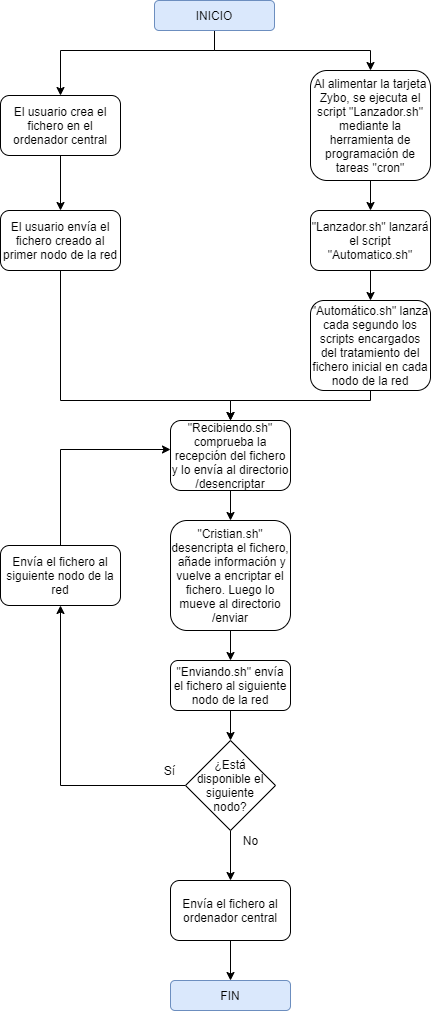
\includegraphics[scale=0.475]{Metodologia/AnalisisSistema/CadenaScripts.png}
%	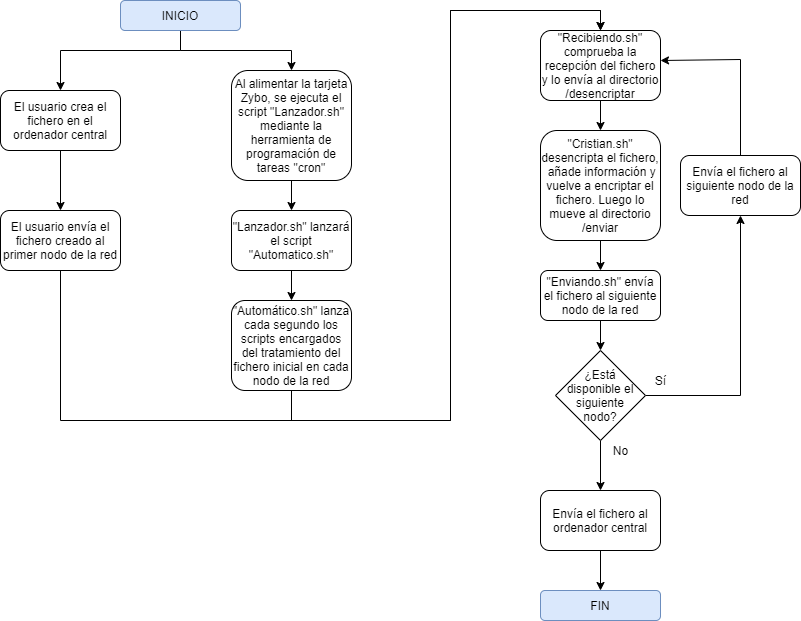
\includegraphics[scale=0.6]{Metodologia/AnalisisSistema/CadenaScriptsAncho.png}
	\caption{Secuencia de trabajo}
	\label{Secuencia de trabajo}
\end{figure}
\newpage
	\chapter{Diseño y desarrollo}

\section{Hardware}
Aquí explicamos lo citado en el apartado de análisis.

\section{Software}
Aquí explicamos lo citado en el apartado de análisis.
	\section{Pruebas del sistema}
%Aquí describimos los scripts para hacer pruebas e incluir las pruebas que hice para ver su funcionamiento.
\subsection{Hardware}
%\textcolor{red}{Prueba de la infraestructura: Lanzar el script Inicio.sh para que se vea que todas las tarjetas dan ping.}
Para realizar la prueba de la arquitectura de red, lanzaremos el script \hyperlink{ScriptConexion}{\texttt{Inicio.sh}}. Este script, nos dirá qué tarjeta está conectada o desconectada de la red.

\begin{figure}[h]
	\centering
	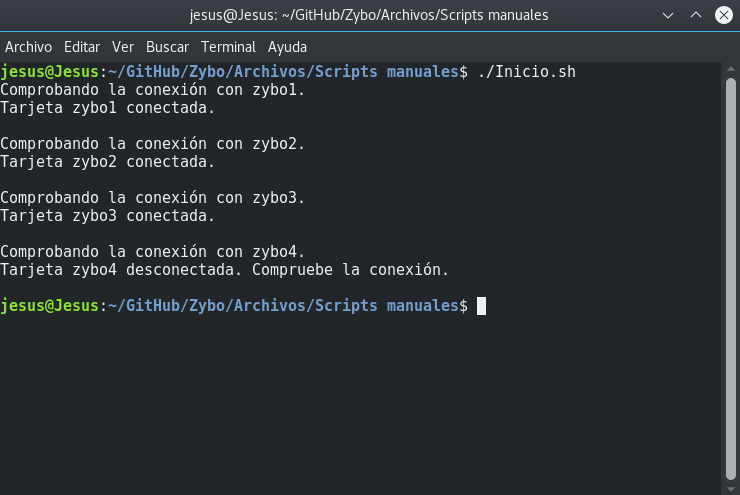
\includegraphics[scale=0.5]{Metodologia/Pruebas/Prueba_Inicio_sh.png}
	\caption{Prueba de \texttt{Inicio.sh}}
	\label{Prueba de Inicio.sh}
\end{figure}

\subsection{Software}
%\textcolor{red}{Prueba de funcionamiento de la recolección de datos: Una prueba de todo funcionando.}
Para realizar las pruebas de funcionamiento, basta con alimentar los nodos participantes en la cadena. En ese momento se ejecuta automáticamente los scripts descritos en el \hyperlink{Scripts}{Apéndice B}. 

Para el correcto funcionamiento de estos scripts, se requiere que el monitor central disponga del fichero inicial de datos creado por el usuario y que dicho usuario lo envíe al primer nodo de la red.

Hecho esto, sucede lo siguiente:
\begin{enumerate}
	\item Envío del fichero inicial a la primera tarjeta: Esto lo haremos gracias a la herramienta \texttt{sshpass} de Linux con la siguiente orden:
	\begin{center}
		\texttt{sshpass -p zyboX scp -o StrictHostKeyChecking=no archivoLocal zyboX@zyboX:/home/zyboX/ficheros/recibir}
	\end{center}
	Este proceso (Figura \ref{Fichero inicial en el ordenador central y envío al primer nodo}) lo podemos ver más detalladamente en el \hyperlink{EnvioRecepcionFicheros}{Apéndce A.4}.
	\begin{figure}[h]
		\centering
		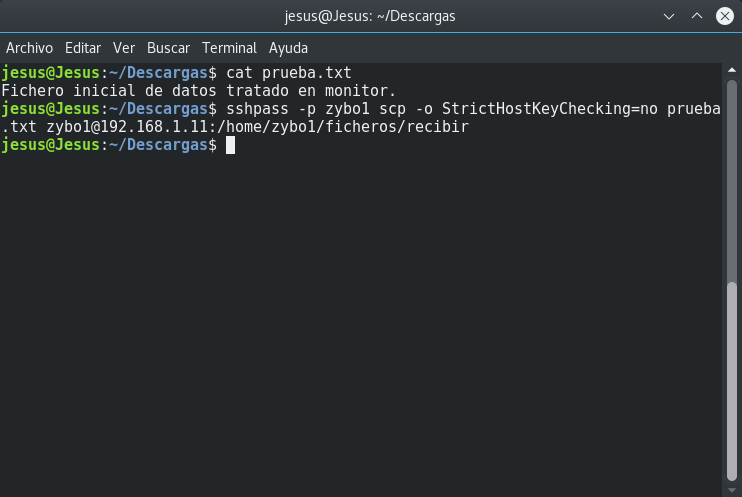
\includegraphics[scale=0.5]{Metodologia/Pruebas/Fichero_inicial_en_PC.png}
		\caption{Fichero inicial en el ordenador central y envío al primer nodo}
		\label{Fichero inicial en el ordenador central y envío al primer nodo}
	\end{figure}
\newpage
	\item Recepción del fichero en las tarjetas: Será el script \hyperlink{ScriptRecibiendo}{\texttt{Recibiendo.sh}} el encargado de comprobar la llegada del fichero y actuar en consecuencia cambiándolo de directorio.

	\item Modificación del fichero: El script \hyperlink{ScriptCristian}{\texttt{Cristian.sh}} será el encargado de abrir el fichero, modificarlo en cada una de las tarjetas y dejarlo preparado para su envío al siguiente nodo de la red. Para comprobar que los resultados de este script son correctos, podemos usar los comandos que vemos en la Figura \ref{Estado del fichero después de su modificación en Zybo1}.
	\begin{figure}[h]
		\centering
		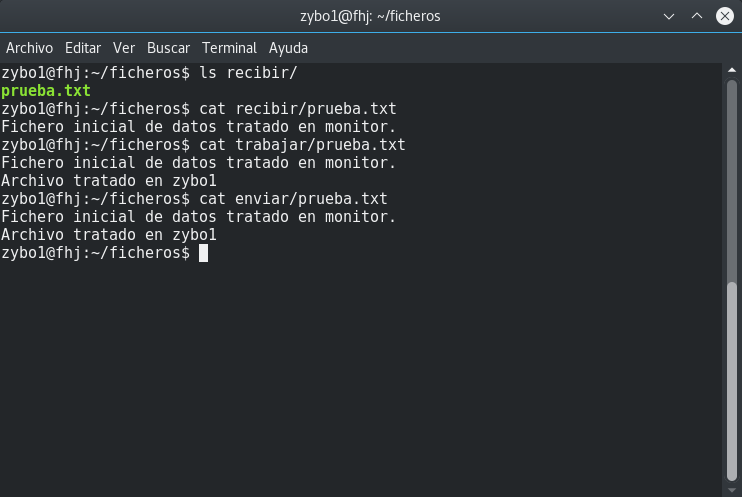
\includegraphics[scale=0.5]{Metodologia/Pruebas/Fichero_en_Zybo1.png}
		\caption{Estado del fichero después de su modificación en Zybo1}
		\label{Estado del fichero después de su modificación en Zybo1}
	\end{figure}
\newpage
	\item Envío del fichero hacia el siguiente nodo: Podemos distinguir dos tipos de envío del mismo fichero. Ambos llevados a cabo por el script \hyperlink{ScriptEnviando}{Enviando.sh}:
	\begin{enumerate}
		\item Tarjeta-Tarjeta: Esta opción se dará cuando la tarjeta actual detecte que la siguiente tarjeta está conectada.
		\item Tarjeta-Ordenador: Esta opción se dará cuando la tarjeta no detecte a la siguiente tarjeta. Entonces, enviará el fichero de datos, de vuelta al ordenador central.
	\end{enumerate}

\newpage
	\item Recepción del fichero en el ordenador central: El fichero final de datos, será recibido en el directorio\\ \texttt{/home/jesus/Vídeos} del ordenador central y contendrá los datos añadidos por todos los nodos de la red.
	\begin{figure}[h]
		\centering
		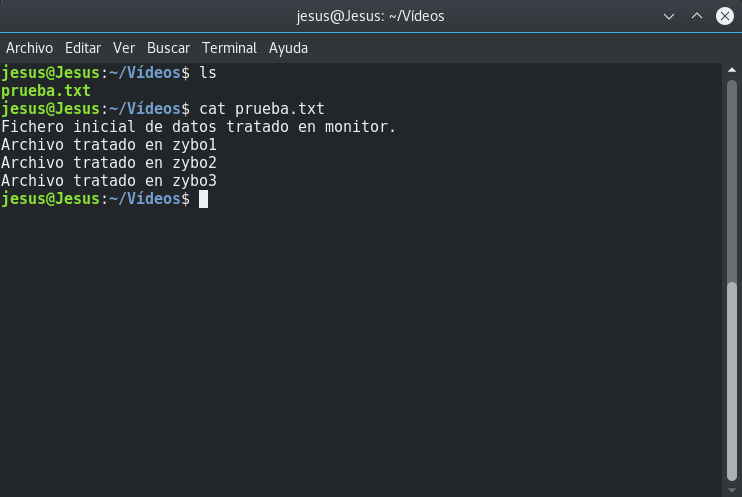
\includegraphics[scale=0.5]{Metodologia/Pruebas/Fichero_final_en_PC.png}
		\caption{Fichero final en el ordenador central}
		\label{Fichero final en el ordenador central}
	\end{figure}

\end{enumerate}

	\part{Conclusiones y trabajo futuro}
	\section{Conclusiones}
Después de las pruebas llevadas a cabo, podemos concluir el proyecto con un enfoque positivo. Gracias a la infraestructura de red creada, se ha conseguido con éxito una recopilación de datos colaborativa partiendo de un fichero inicial de datos desde el ordenador central, pasando por todos los nodos de la red y llegando, de nuevo, al ordenador central.

Además se ha conseguido que la información aportada por cada uno de los nodos de la red, está desligada de su dirección IP, de forma que, a priori, no se conozca la información que añadió cada nodo. El único inconveniente de esto es que, al ser una cadena secuencial, solo tendremos que saber qué nodos están conectados a la red para saber la información añadida por cada nodo.

Se pueden destacar varios escenarios de trabajo:
\begin{itemize}
	\item Si todos los nodos están conectados correctamente a la red, se producirá un recorrido lineal que partirá desde el ordenador central, viajará por todos los nodos desde zybo1 hasta zyboX. Una vez que se recorra toda la cadena y, al no detectar el siguiente nodo, zybo(X+1), el fichero retornará al ordenador central.
	\begin{figure}[h]
		\centering
		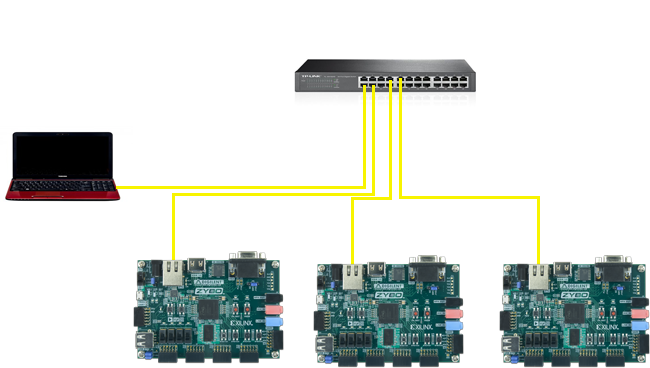
\includegraphics[scale=0.5]{Epilogo/RedCompleta.png}
		\caption{Red completa}
		\label{Red completa}
	\end{figure}
\newpage
	\item Cuando algún nodo intermedio de la red está desconectado, la cadena se romperá y, el nodo anterior, al no conseguir comunicación, enviará el fichero con la información recopilada al ordenador central, obviando el resto de nodos.
	\begin{figure}[h]
		\centering
		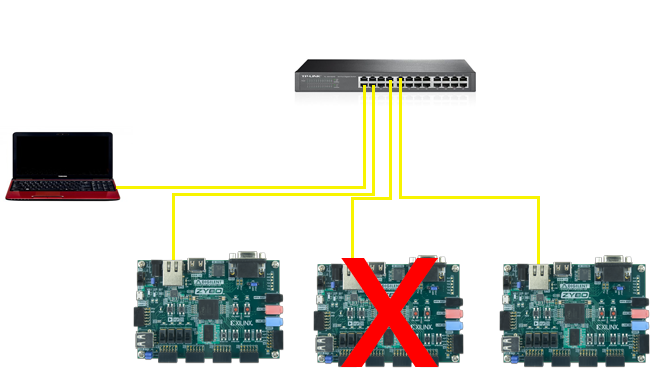
\includegraphics[scale=0.5]{Epilogo/RedSinNodo2.png}
		\caption{Red sin nodo intermedio}
		\label{Red sin nodo intermedio}
	\end{figure}
%\newpage
	\item Otro escenario será cuando el primer nodo de la red está desconectado.
	\begin{figure}[h]
		\centering
		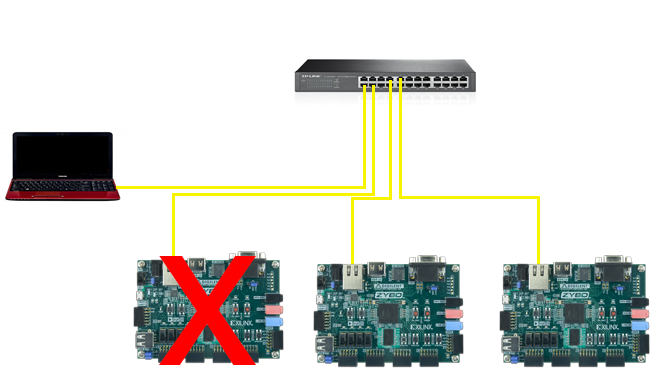
\includegraphics[scale=0.5]{Epilogo/RedSinNodo1.png}
		\caption{Red sin primer nodo}
		\label{Red sin primer nodo}
	\end{figure}\\
	Entonces, tendremos dos opciones:
	\begin{itemize}
		\item Volver a revisar la conexión con el primer nodo hasta conseguir solucionar el problema.
		\item Usar como primer nodo el segundo, enviando el fichero inicial directamente al segundo nodo de la red.
	\end{itemize}
\end{itemize}

Como ejemplo práctico de aplicación de esta red, se planteó como objetivo que la información aportada localmente por cada nodo fuera cifrada mediante un IP cifrador/descifrador AES \hyperlink{1}{[1]}. Para llevar a cabo esta aplicación, era necesario contar con el driver incluido en el sistema operativo compilado en otro Trabajo de Fin de Grado \hyperlink{2}{[2]}. A causa de la incompatibilidad de dicho sistema operativo compilado y los modelos de tarjeta Zybo utilizados en ambos proyectos, este objetivo no se ha podido completar.

\section{Trabajo futuro}
Como trabajo futuro quedaría cambiar la cadena de conexiones y que, en vez de recorrer los nodos de forma secuencial, se hiciera de forma aleatoria, para que no se supiera qué nodo ha seguido a cual. De esta forma, se conseguirá un desconocimiento total por parte del ordenador central sobre qué nodo añadió cada información al fichero final.

Para completar el trabajo de cifrado/descifrado de datos en la cadena de nodos de la red, deberíamos encontrar la compatibilidad con el sistema operativo aportado por el Trabajo de Fin de Grado de Gabriel Fernando Sánchez Reina. Una vez tengamos dicha compatibilidad y, debido a que dicho sistema operativo incluye el IP cifrador/descifrador de Cristian Ambrosio Costoya, ya podríamos realizar el cifrado/descifrado de los ficheros enviados por la red.

Otro posible uso de la red sería el tratamiento de una imagen, de modo que un IP dedicado a esto, formara parte del nodo de red.

También se podría mejorar el proyecto incluyendo un módulo Wi-Fi, de modo que los nodos, no tengan que estar necesariamente conectados por cable. Esto nos daría la posibilidad de ubicar cada nodo donde quisiéramos (dentro de las capacidades físicas de la red Wi-Fi) y así poder usar dicha estructura en un entorno de IoT\footnote{Internet of Things.} para una casa o el edificio que necesitemos. Para este cambio no haría falta modificar nada del software aportado por este proyecto.

	
	\part{Referencias/Bibliografía}
	%\textcolor{red}{Aquí empezaré a poner la bibliografía que constará de los foros y las páginas web que se han ido consultando a la hora de realizar el proyecto.}
%\begin{itemize}
\hspace{0.5cm}	[\hypertarget{1}{1}] IP cifrador/descifrador como Trabajo de Fin de Grado de Cristian Ambrosio Costoya. %Consultado el 20/02/2020.

\hspace{0.5cm}	[\hypertarget{2}{2}] Interfaz de conexión entre Linux y el IP cifrador/descifrador como Trabajo de Fin de Grado de Gabriel Fernando Sánchez Reina. %Consultado el 20/02/2020.

\hspace{0.5cm}	[\hypertarget{3}{3}] Manual de referencia oficial de DIGILENT: \url{https://reference.digilentinc.com/_media/zybo:zybo_rm.pdf}. Consultado el 15/05/2019.

\hspace{0.5cm}	[\hypertarget{4}{4}] Manual de SSH: \url{https://linux.die.net/man/1/ssh}. Consultado el 03/06/2019.

\hspace{0.5cm}	[\hypertarget{5}{5}] Manual de la herramienta \texttt{dd}: \url{https://man7.org/linux/man-pages/man1/dd.1.html}. Consultado el 20/08/2020.

\hspace{0.5cm}	[\hypertarget{6}{6}] Manual de la herramienta sshpass: \url{https://linux.die.net/man/1/sshpass}. Consultado el 10/06/2019.

\hspace{0.5cm}	[\hypertarget{7}{7}] Manual de scp: \url{https://linux.die.net/man/1/scp}. Consultado el 04/06/2019.

\hspace{0.5cm}	[\hypertarget{8}{8}] Compresión y descompresión de ficheros \url{http://ecapy.com/comprimir-y-descomprimir-tgz-} \url{tar-gz-y-zip-por-linea-de-comandos-en-linux/index.html}. Consultado el 20/05/2019.

\hspace{0.5cm}	[\hypertarget{9}{9}] Manual de stat: \url{https://linux.die.net/man/2/stat}. Consultado el 29/05/2019.

\hspace{0.5cm}	[\hypertarget{10}{10}] Manual de crontab: \url{https://linux.die.net/man/1/crontab}. Consultado el 03/06/2019.
	
\hspace{0.5cm}	[\hypertarget{11}{11}] Creación de diagramas de flujo gracias a la herramienta \url{https://app.diagrams.net/}. Consultado el 29/05/2019.
	
\hspace{0.5cm}	[\hypertarget{12}{12}] Clonación de tarjetas SD en Linux: \url{https://www.altaruru.com/como-clonar-una-sd-}\\
	\url{raspberry-pi-orange-pi/}. Consultado el 20/08/2020.

\hspace{0.5cm}	[\hypertarget{13}{13}] Protocolo SSH: \url{https://es.wikipedia.org/wiki/Secure_Shell} Consultado el 03/06/2019.
%\end{itemize}
	
	\part{Anexos técnicos}
	\appendix
	\chapter{Manual de usuario}
Aquí puedo poner mis manuales.

	\chapter{Datos técnicos}
Aquí puedo poner algún dato técnico a tener en cuenta en el proyecto.
	\chapter{Scripts}
\hypertarget{Scripts}{}
%Aquí puedo incrustar tal cual los scripts del proyecto.
En este apéndice, describiremos los distintos scripts que podemos encontrar en las tarjetas Zybo con su explicación y código correspondiente.

Dicha descripción se hará siguiendo el orden que recorrerá el archivo recibido desde el dispositivo anterior hasta ser enviado al siguiente dispositivo.

Para comprobar el estado de todos los directorios, usaremos el comando \texttt{stat} para comprobar el estado de los directorios.

En el trabajo aquí mencionado se emula el desencriptado de un fichero, adición de información, cifrado, y envío del mismo a otro dispositivo\footnote{Para cambiar dicho comportamiento, solo tendremos que modificar los scritps que se encargan de automatizar el proceso.}. \textcolor{red}{Esto habría que cambiarlo puesto que ahora sí que tenemos el trabajo de Cristian.}

\newpage
\section{\texttt{Inicio.sh}}
\hypertarget{ScriptConexion}{}
El script se encarga de probar las conexiones de todos los dispositivos de la red para ver que están conectados al switch.

\subsection{Diagrama de flujo}
\begin{figure}[h]
	\centering
	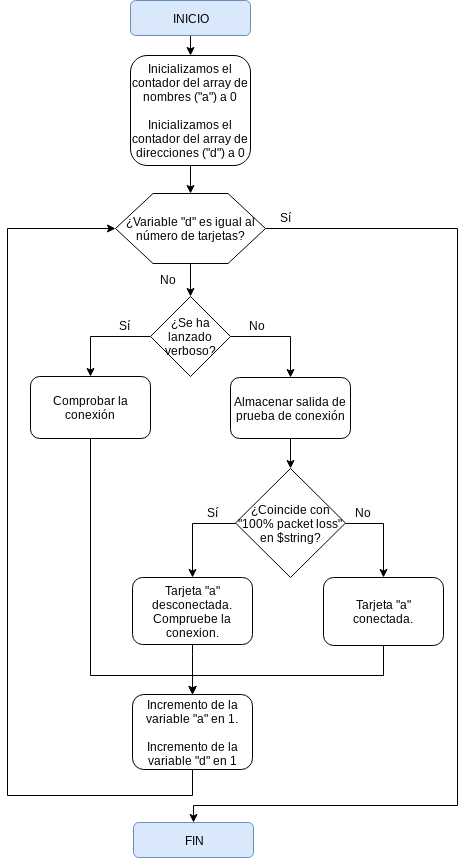
\includegraphics[scale=0.562]{Anexos/Anexo2/Test/Inicio.png}
	\caption{Diagrama de flujo de \texttt{Inicio.sh}}
	\label{Diagrama de flujo de Inicio.sh}
\end{figure}

\newpage
\subsection{Código}
\lstinputlisting[language=Bash]{Anexos/Anexo2/Test/Inicio.sh}
\begin{center}
	Código de \texttt{Inicio.sh} usando cuatro tarjetas como ejemplo.
\end{center}


\section{\texttt{Lanzador.sh}}
\hypertarget{ScriptLanzador}{}
Este script se encarga de lanzar el script \texttt{Automatico.sh} mediante la herramienta cron\footnote{Para más información, ver el manual de crontab en este \href{https://linux.die.net/man/5/crontab}{\textcolor{blue}{enlace}}.} al inicio del sistema operativo Xillinux.

Para usarlo, debemos usar el siguiente comando:
\begin{center}
	\texttt{crontab -e}
\end{center}

Y, luego, añadir la regla que queramos que se ejecute al final del fichero. En nuestro caso es la siguiente:
\begin{center}
	\texttt{@reboot (cd \textasciitilde/ficheros; ./Lanzador.sh)}
\end{center}

Esto hará que la herramienta cron inicie este script al iniciar el sistema operativo Xillinux de las tarjetas Zybo.

\newpage
\subsection{Diagrama de flujo}
\begin{figure}[h]
	\centering
	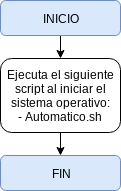
\includegraphics[scale=0.9]{Anexos/Anexo3/Diagramas/Lanzador.png}
	\caption{Diagrama de flujo de \texttt{Lanzador.sh}.}
	\label{Diagrama de flujo de Lanzador.sh}
\end{figure}

\subsection{Código}
\lstinputlisting[language=Bash]{Anexos/Anexo3/Scripts/Lanzador.sh}
\begin{center}
	Código de \texttt{Lanzador.sh}.
\end{center}


\newpage
\section{\texttt{Automatico.sh}}
\hypertarget{ScriptAutomatico}{}
Este script es el encargado de lanzar el resto de scripts periódicamente para que vayan comprobando los directorios correspondientes y se produzca la comunicación de forma automática.

%\newpage
\subsection{Diagrama de flujo}
\begin{figure}[h]
	\centering
	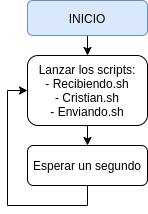
\includegraphics[scale=0.9]{Anexos/Anexo3/Diagramas/Automatico.png}
	\caption{Diagrama de flujo de \texttt{Automatico.sh}.}
	\label{Diagrama de flujo de Automatico.sh}
\end{figure}

\subsection{Código}
\lstinputlisting[language=Bash]{Anexos/Anexo3/Scripts/Automatico.sh}
\begin{center}
	Código de \texttt{Anexos/Anexo3/Automatico.sh}.
\end{center}


\newpage
\section{\texttt{Recibiendo.sh}}
\hypertarget{ScriptRecibiendo}{}
Este script es el encargado de comprobar el estado del directorio \texttt{\textasciitilde/ficheros/recibir} y, si llega un archivo nuevo, enviarlo al directorio \texttt{\textasciitilde/ficheros/desencriptar}.

%\newpage
\subsection{Diagrama de flujo}
\begin{figure}[h]
	\centering
	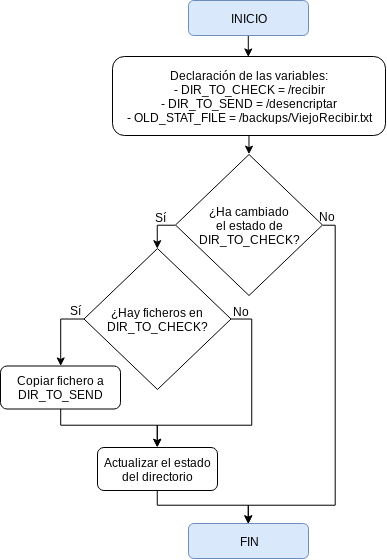
\includegraphics[scale=0.8]{Anexos/Anexo3/Diagramas/Recibiendo.png}
	\caption{Diagrama de flujo de \texttt{Recibiendo.sh}.}
	\label{Diagrama de flujo de Recibiendo.sh}
\end{figure}

\subsection{Código}
\lstinputlisting[language=Bash]{Anexos/Anexo3/Scripts/Recibiendo.sh}
\begin{center}
	Código de \texttt{Recibiendo.sh}.
\end{center}

\section{\texttt{Cristian.sh}}
\hypertarget{ScriptCristian}{}
\textcolor{red}{A este script le pondré el nombre \texttt{Encriptando.sh} seguramente, porque básicamente se encargará de eso (tanto encriptar como desencriptar), o, a unas malas, le pongo \texttt{Trabajando.sh}. También tengo la opción de hacer dos, uno que encripte y otro que desencripte, depende de como vea que funciona una vez que tenga las tarjetas. Así que, hasta que no tenga las tarjetas y me ponga a hacer las pruebas de verdad con todo (tanto lo de Gabri como lo de Cristian, esta parte queda un poco en el aire para perfeccionarla luego.).}

Este script es el encargado de emular el trabajo de nuestro compañero Cristian y realiza las siguientes tareas:
\begin{itemize}
	\item Gracias al crontab establecido, se encarga de comprobar periódicamente el estado del directorio \texttt{\textasciitilde/ficheros/desencriptar}.
	\item Mueve el archivo allí situado al directorio \texttt{\textasciitilde/ficheros/trabajar} (simulando el desencriptado del mismo).
	\item Una vez allí, añade un texto como el siguiente:
	\begin{center}
		\texttt{Archivo tratado en zyboX}
	\end{center}	
	Siendo zyboX el identificador de la tarjeta con la que estamos trabajando.
	\item Por último, envía el fichero al directorio \texttt{\textasciitilde/ficheros/enviar}.
\end{itemize}

\newpage
\subsection{Diagrama de flujo}
\begin{figure}[h]
	\centering
	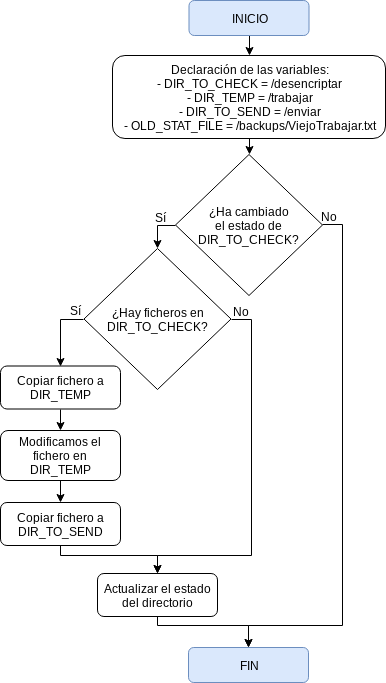
\includegraphics[scale=0.7]{Anexos/Anexo3/Diagramas/Cristian.png}
	\caption{Diagrama de flujo de \texttt{Cristian.sh}.}
	\label{Diagrama de flujo de Cristian.sh}
\end{figure}

\newpage
\subsection{Código}
\lstinputlisting[language=Bash]{Anexos/Anexo3/Scripts/Cristian.sh}
\begin{center}
	Código de \texttt{Cristian.sh}.
\end{center}

\newpage
\section{\texttt{Enviando.sh}}
\hypertarget{ScriptEnviando}{}
Este script es el encargado de comprobar periódicamente el estado del directorio\\ \texttt{\textasciitilde/ficheros/enviar} y, cuando detecta un cambio, envía el archivo a la siguiente tarjeta, o, si ésta se encuentra desconectada, al ordenador central.

A la hora de comprobar si la siguiente tarjeta está conectada o no, se hace enviando un comando ping a la siguiente tarjeta, por lo que se nos presentarán dos posibles casos:
\begin{itemize}
	\item \textbf{Éxito:} La tarjeta está conectada y será allí donde se envíe el fichero.
	\item \textbf{Fracaso:} La tarjeta no está conectada y el fichero será enviado al ordenador central.
\end{itemize}

Para que podamos usar el comando ping desde este script, debemos darle permisos de ejecución en modo usuario de la siguiente forma:
\begin{enumerate}
	\item Entramos como super-usuario con el comando \texttt{su} y contraseña \texttt{zyboX} (siendo X el identificador de la tarjeta con la que estamos trabajando).
	\item A continuación, introducimos el siguiente comando:
	\begin{center}
		\texttt{chmod u+s /bin/ping}
	\end{center}
	Y con eso, quedaría activado el comando \texttt{ping} para poder usarlo desde este script.
\end{enumerate}

\newpage
\subsection{Diagrama de flujo}
\begin{figure}[h]
	\centering
	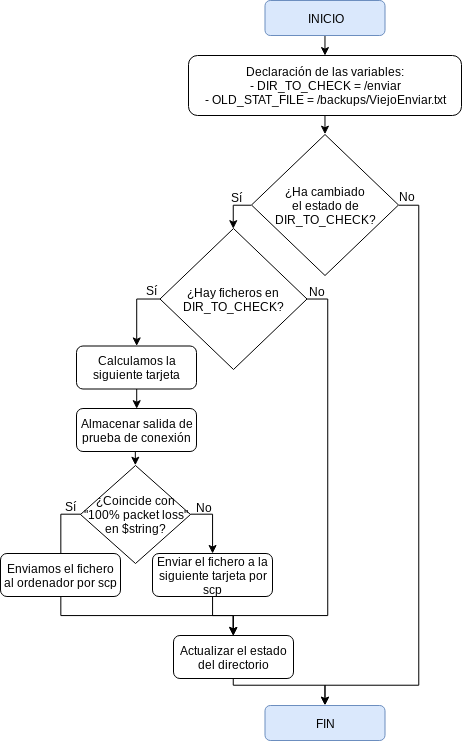
\includegraphics[scale=0.65]{Anexos/Anexo3/Diagramas/Enviando.png}
	\caption{Diagrama de flujo de \texttt{Diagramas/Enviando.sh}.}
	\label{Diagrama de flujo de Enviando.sh}
\end{figure}

\newpage
\subsection{Código}
\lstinputlisting[language=Bash]{Anexos/Anexo3/Scripts/Enviando.sh}
\begin{center}
	Código de \texttt{Enviando.sh}.
\end{center}


\section{\texttt{Borrar.sh}}
\hypertarget{ScriptBorrar}{}
Este script se encarga de borrar el contenido de los directorios \texttt{\textasciitilde/ficheros/recibir},\\ \texttt{\textasciitilde/ficheros/desencriptar}, \texttt{\textasciitilde/ficheros/trabajar} y \texttt{\textasciitilde/ficheros/enviar} de las tarjetas Zybo.

Para ejecutarlo solo debemos usar el siguiente comando en el directorio \texttt{\textasciitilde/ficheros} de las tarjetas Zybo:
\begin{center}
	\texttt{./Borrar.sh}
\end{center}

\subsection{Diagrama de flujo}
\begin{figure}[h]
	\centering
	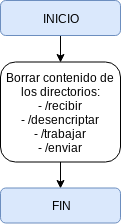
\includegraphics[scale=0.9]{Anexos/Anexo3/Diagramas/Borrar.png}
	\caption{Diagrama de flujo de \texttt{Borrar.sh}.}
	\label{Diagrama de flujo de Borrar.sh}
\end{figure}

%\newpage
\subsection{Código}
\lstinputlisting[language=Bash]{Anexos/Anexo3/Scripts/Borrar.sh}
\begin{center}
	Código de \texttt{Borrar.sh}.
\end{center}
	
\end{document}
